\section{Technik}


\subsection{Grundlagen}
\begin{frame}
\frametitle{Ein typisches Freifunk Netz}
    \begin{itemize}
        \item Ein Batman-Adv Netz
        \begin{itemize}
            \item \glqq Wie ein großer dezentraler Switch\grqq 
        \end{itemize}
        \item VPN (fastd)/L2TP für die Funkinseln
        \begin{itemize}
            \item Multi-Client zu Multi-Client VPN
            \item Kein internes Routing
            \item Kein Forwarding
            \item Layer-II Netz
        \end{itemize}
        \item Mehrere VPN Server / Gateway
        \begin{itemize}
            \item DHCP
            \item DNS Namensauflösung
            \item Gateway zum Internet / ICVPN
            \begin{itemize}
                \item z.B. mittels Policy-based routing
            \end{itemize}
        \end{itemize}
        \item Monitoring
        \begin{itemize}
            \item Karte aller Knoten
        \end{itemize}
    \end{itemize}
\end{frame}

\begin{frame}
\frametitle{Freifunk Router (aussen)}
    \begin{itemize}
        \item Client-Ports \& Infrastructure Funknetz:
            Wie ein großer Switch
        \item Batman-Ports \& Ad-Hoc Funknetz:
            Mesh-Netz
        \item WAN-Ports:
            VPN Netz
    \end{itemize}
    \center{
        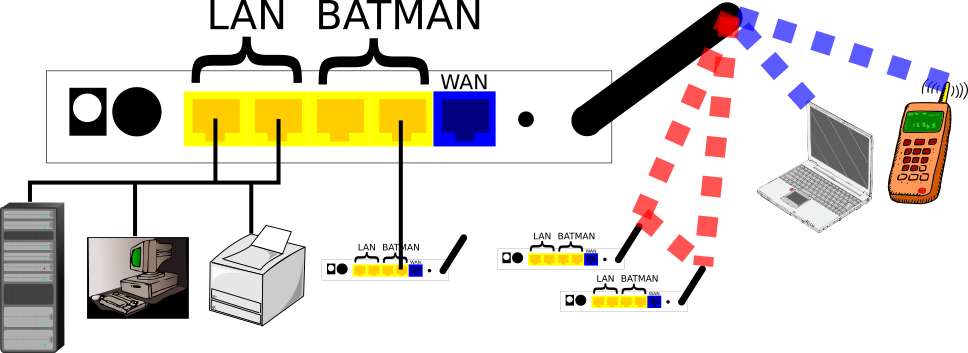
\includegraphics[width=0.75\textwidth]{images/anschluesse.png}
    }
\end{frame}

\begin{frame}
\frametitle{Freifunk Router (innen)}
    \begin{itemize}
        \item OpenWrt
        \item Batman-Adv
        \item Fastd Client / L2TP zum Gateway
        \item Monitoring Daten (Nodewatcher / Alfred)
        \item .. kleinere Tools / Configs / Skripte
    \end{itemize}

    \renewcommand{\arraystretch}{1.5}
    \begin{tabular}{|c|c|c|c|c|c|c|} \hline
         \multicolumn{7}{|c|}{Bridge} \\ \hline
         \multirow{2}{*}{Managed} &
         \multicolumn{4}{c|}{B.A.T.M.A.N} &
         \multicolumn{2}{c|}{\multirow{2}{*}{Client-VLan}} \\ \cline{2-5}
         & Ad-Hoc & VPN & \multicolumn{2}{c|}{Node-VLan} & \multicolumn{2}{c|}{} \\ \hline
         \multicolumn{2}{|c|}{WiFi} & WAN & LAN1 & LAN2 &
         LAN3 & LAN4 \\ \hline
    \end{tabular}
\end{frame}

\begin{frame}
\frametitle{Ein typisches Freifunk Netz}
    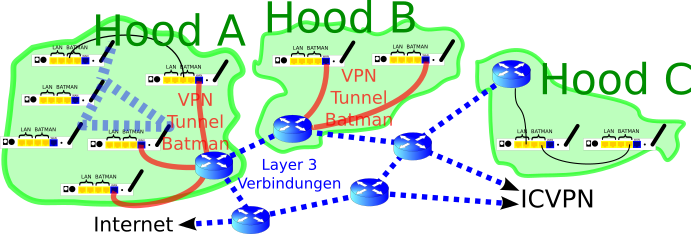
\includegraphics[width=\textwidth]{images/freifunk_konzepte.png}

    \begin{itemize}
        \item Mehrere Layer-2 Inseln (Hoods)
        \item Verbindung per Layer-3
        \item Dezentrale Gateways
    \end{itemize}
\end{frame}




\subsection{Stand von heute}

\begin{frame}
\frametitle{Freifunk Knoten}
    \begin{itemize}
        \item Ziel: Ohne große Konfiguration
        \begin{itemize}
            \item Keine DHCP Ranges
            \item LAN Ports vorkonfiguriert
            \item Ausnahme: Passwort für root Login und Standort
        \end{itemize}
        \item Hat nur eine Link-Local IPv6 Adresse
        \item Webconfig und SSH-Config
        \item Batman-Adv
    \end{itemize}
\end{frame}

\begin{frame}
\frametitle{Knoten VPN}
    \begin{itemize}
        \item Verwendetes VPN: fastd oder L2TP
        \item Wir nutzen keine Verschlüsselung (! :-O)
        \item Script zum Austausch der VPN Peers über den KeyXchange
    \end{itemize}
\end{frame}

\begin{frame}
\frametitle{VPN-KeyXchange}
    \begin{itemize}
        \item Zentrale Webseite
        \item Knoten meldet sich beim VPN-KeyXchange an
        \item Knoten lädt Liste mit Server
        \item Knoten Identifizierung über MAC, alternativ über Name
        \item<2> Aufteilung in ,,hood''s:
        \begin{itemize}
            \item Die Hood, welche am nächsten dran ist wird zugewiesen
            \item Clients bekommen eine Liste aller Server
            \item Server bekommen eine Liste aller Clients+Server
        \end{itemize}
        \item<2> Problem: Funk Verbindung zwischen den Hoods
    \end{itemize}
\end{frame}

\begin{frame}
\frametitle{VPN Server}
    \begin{itemize}
        \item VPN Server: In jeder Hood gibt es mehrere davon
        \item Hoodzuweisung manuell im KeyXchange
        \item DHCP
        \begin{itemize}
            \item Aktuell ausschließlich IPv4
            \item Ungleiche Server Auslastung durch schlechtes DHCP Timing
            \item Batman-Adv GW Selection
        \end{itemize}
        \item DNS Namesauflösung
        \item Policy base routing
        \item VPN (GRE) Tunnel zu anderen Gateways
        \item Babel
        \begin{itemize}
            \item Routing zu anderen Gateways
        \end{itemize}
    \end{itemize}
\end{frame}

\begin{frame}
\frametitle{Gateways}
    \begin{itemize}
        \item Verbindet Freifunk und Internet
        \item IPv4 NAT (oft übers Ausland) ins Internet
        \item Announced 0.0.0.0/0 via Babel
    \end{itemize}
\end{frame}



\begin{frame}
\frametitle{Monitoring}
    \begin{itemize}
        \item Alfred
        \begin{itemize}
            \item XML
            \item alle 5 Minuten
            \item Multicast
        \end{itemize}
        \item Multicast Daten können auf mehreren Gateways gelesen werden
        \item Die Daten können von dort an eine zentrale Webseite (Karte, etc.) geschickt werden
        \item Standort und Ansprechpartner wird über Alfred geladen
    \end{itemize}
\end{frame}

\begin{frame}
\frametitle{Domain-Name-System}
    \begin{itemize}
        \item fff.community
        \begin{itemize}
            \item Langer Name, aber
            \item Keine Kollision
        \end{itemize}
        \item Mehrere DNS Server
        \item Zonen-Synchronisation über dig axfr
        \item Subdelegation an synchronisierte Hosts möglich
    \end{itemize}
\end{frame}

\begin{frame}
\frametitle{Firmware Bau}
    \begin{itemize}
        \item Basiert auf OpenWrt
        \item ,,Eigenes'' Framework (Buildscript)
        \item Board-Support-Packages
        \begin{itemize}
            \item Ein .config
            \item Überschreibende ,,files''
        \end{itemize}
        \item Template System für versch. Communities
    \end{itemize}
\end{frame}

\begin{frame}
\frametitle{Zusammenfasssung}
    \begin{itemize}
        \item Erfolgreich das L2 Netz in mehrere L3 Netze geteilt
        \item VPN Schlüsseltausch über zentrales Tool
        \begin{itemize}
            \item Manuelle Zuweisung der VPN Server
            \item Keine Anpassung an Firmware
            \begin{itemize}
                \item Fehlerhafte Verbindung (loop) der Hoods durch versehentliches Meshing
            \end{itemize}
        \end{itemize}
        \item Kein Traffic Balancing zwischen VPN Server und Gateways
    \end{itemize}
\end{frame}


\begin{frame}
\frametitle{Weathermap}

    \center{
        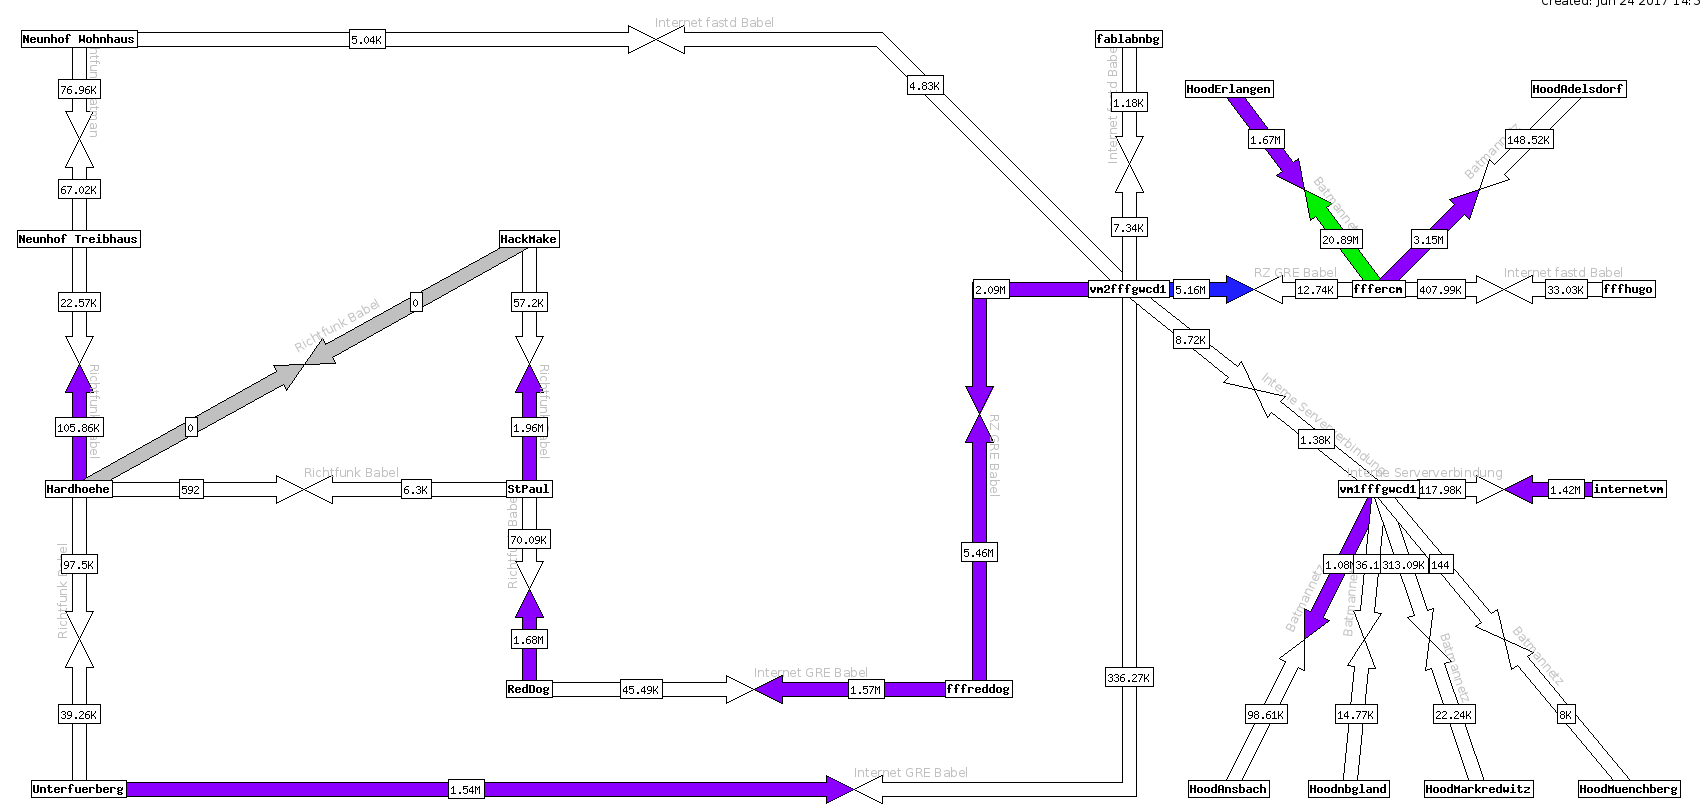
\includegraphics[width=\textwidth]{images/richtfunk.png}
    }
\end{frame}